\newif\ifalone
\alonefalse
\newif\iftalk
\talktrue

\ifalone
\documentclass{article}
\usepackage{graphicx}
\usepackage{natbib}
\usepackage{amsfonts}
\usepackage{amssymb}
\usepackage{amsthm}
\usepackage{bm}
\usepackage{Sweave}
\usepackage{lscape}
\usepackage{makeidx}
\usepackage{color}

\title{GLMs and GLMMs}

\author{Jarrod Hadfield (\texttt{j.hadfield@ed.ac.uk})}
\begin{document}
\maketitle
\else
\chapter[GLMM]{Generalised Linear Mixed Models (GLMM)}
\label{chap2}
\fi



\section{Linear Model (LM)}

A linear model is one in which unknown parameters are multiplied by observed variables and then added together to give a prediction for the response variable. As an example, lets take the results from a Swedish experiment from the sixties:

\begin{Schunk}
\begin{Sinput}
> data(Traffic, package = "MASS")
> Traffic$year <- as.factor(Traffic$year)
> Traffic[c(1, 2, 184), ]
\end{Sinput}
\begin{Soutput}
    year day limit  y
1   1961   1    no  9
2   1961   2    no 11
184 1962  92   yes  9
\end{Soutput}
\end{Schunk}

The experiment involved enforcing speed limits on Swedish roads on some days, but on other days letting everyone drive as fast as they liked.  The response variable (\texttt{y}) was how many of their citizens were injured in road accidents! The experiment was conducted in 1961 and 1962 for 92 days in each year. As a first attempt we could specify the linear model:

\begin{Schunk}
\begin{Soutput}
y ~ limit + year + day
\end{Soutput}
\end{Schunk}

but what does this mean?\\

\subsection{Linear Predictors}
\label{lm-sec}

The model formula defines a set of simultaneous (linear) equations 

\begin{displaymath}
\begin{array}{cl}
E[y\texttt{[1]}] &=\beta_{1}+\beta_{2}(\texttt{limit[1]=="yes"})+\beta_{3}(\texttt{year[1]=="1962"})+\beta_{4}\texttt{day[1]}\\
E[y\texttt{[2]}] &= \beta_{1}+\beta_{2}(\texttt{limit[2]=="yes"})+\beta_{3}(\texttt{year[2]=="1962"})+\beta_{4}\texttt{day[2]}\\
\vdots&=\vdots\\
E[y\texttt{[184]}] &= \beta_{1}+\beta_{2}(\texttt{limit[184]=="yes"})+\beta_{3}(\texttt{year[184]=="1962"})+\beta_{4}\texttt{day[184]}\\
\end{array}
\label{SE-eq}
\end{displaymath}

where the $\beta$'s are the unknown coefficients to be estimated, and the variables in \texttt{this font} are observed predictors. Continuous predictors such as \texttt{day} remain unchanged, but categorical predictors are expanded into a series of binary variables of the form `\emph{do the data come from 1961, yes or no?}', `\emph{do the data come from 1962, yes or no?}', and so on for as many years for which there are data.\\ 

It is cumbersome to write out the equation for each data point in this way, and a more compact way of representing the system of equations is

\begin{equation}
E[{\bf y}] = {\bf X}{\bm \beta}
\label{lm-eq}
\end{equation}	

where ${\bf X}$ is called a design matrix and contains the predictor information, and ${\bm \beta} = [\beta_{1}\ \beta_{2}\ \beta_{3}\ \beta_{4}]^{'}$ is the vector of parameters. 

\begin{Schunk}
\begin{Sinput}
> X <- model.matrix(y ~ limit + year + day, data = Traffic)
> X[c(1, 2, 184), ]
\end{Sinput}
\begin{Soutput}
    (Intercept) limityes year1962 day
1             1        0        0   1
2             1        0        0   2
184           1        1        1  92
\end{Soutput}
\end{Schunk}

The binary predictors \emph{do the data come from 1961, yes or no?} and \emph{there was no speed limit, yes or no?} do not appear. These are the first factor levels of \texttt{year} and \texttt{limit} respectively, and are absorbed into the global intercept ($\beta_{1}$) which is fitted by default in R.  Hence the expected number of injuries for the four combinations (on day zero) are $\beta_{1}$ for 1961 with no speed limit, $\beta_{1}+\beta_{2}$ for 1961 with a speed limit, $\beta_{1}+\beta_{3}$ for 1962 with no speed limit and  $\beta_{1}+\beta_{2}+\beta_{3}$ for 1962 with a speed limit.\\

The simultaneous equations defined by Equation (\ref{lm-eq}) cannot be solved directly because we do not know the expected value of y. We only know the observed value, which we assume is distributed around the expected value with some error. In a normal linear model we assume that these errors are normally distributed so that the data are also normally distributed (after taking into account the predictor variables):

\begin{equation}
{\bf y} \sim N({\bf X}{\bm \beta}, \sigma^{2}_{e}{\bf I})
\end{equation}	

${\bf I}$ is an identity matrix. It has ones along the diagonal, and zeros in the off-diagonals. The zero off-diagonals imply that the residuals are uncorrelated, and the ones along the diagonal imply that they have the same variance  $\sigma^{2}_{e}$. We could use \texttt{glm} to estimate ${\bf \beta}$ and  $\sigma^{2}_{e}$ assuming that y is normally distributed: 

\begin{Schunk}
\begin{Sinput}
> m2a.1 <- glm(y ~ limit + year + day, data = Traffic)
\end{Sinput}
\end{Schunk}

but the injuries are count data and the residuals show the typical right skew:

\iftalk
\else
\begin{Schunk}
\begin{Sinput}
> hist(m2a.1$resid)
\end{Sinput}
\end{Schunk}
\fi


\begin{figure}[!h]
\begin{center}
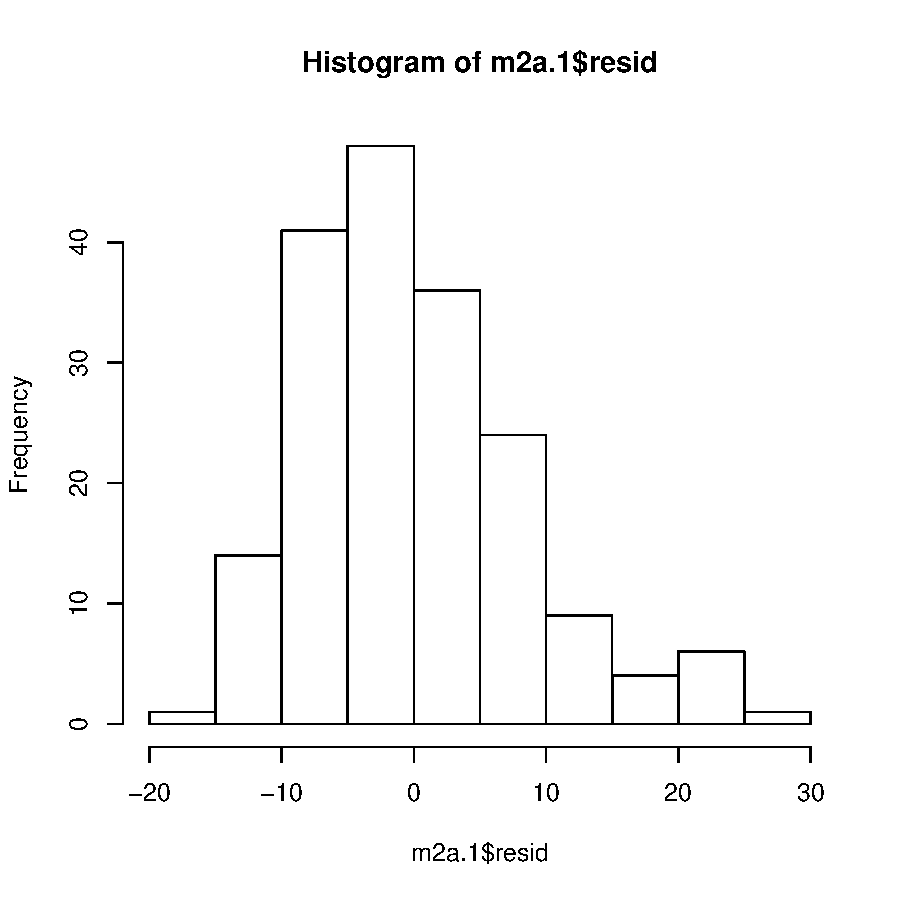
\includegraphics{Lecture2-007}
\end{center}
\caption{Histogram of residuals from model \texttt{m2a.1} which assumed they followed a Gaussian distribution.}
\label{mcmc.traffic-fig}
\end{figure}

Its not extreme, and the conclusions probably won't change, but we could assume that the data follow some other distribution.
 
\section{Generalised Linear Model (GLM)}

Generalised linear models extend the linear model to non-Gaussian data. They are essentially the same as the linear model described above, except they differ in two aspects. First, it is not necessarily the mean response that is predicted, but some function of the mean response. This function is called the link function. For example, with a log link we are trying to predict the logged expectation:

\begin{equation}
\textrm{log}(E[{\bf y}]) = {\bf X}{\bm \beta}
\end{equation}

or alternatively

\begin{equation}
E[{\bf y}] = \textrm{exp}({\bf X}{\bm \beta})
\end{equation}

where \textrm{exp} is the inverse of the log link function. The second difference is that many distributions are single parameter distributions for which a variance does not need to be estimated, because it can be inferred from the mean. For example, we could assume that the number of injuries are Poisson distributed, in which case we also make the assumption that the variance is equal to the expected value.  There are many different types of distribution and link functions and those supported by \texttt{MCMCglmm} can be found in Table \ref{dist-tab}. For now we will concentrate on a Poisson GLM with log link (the default link function for the Poisson distribution):

\begin{Schunk}
\begin{Sinput}
> m2a.2 <- glm(y ~ limit + year + day, family = poisson, data = Traffic)
> summary(m2a.2)
\end{Sinput}
\begin{Soutput}
Call:
glm(formula = y ~ limit + year + day, family = poisson, data = Traffic)

Deviance Residuals: 
    Min       1Q   Median       3Q      Max  
-4.1774  -1.4067  -0.4040   0.9725   4.9920  

Coefficients:
              Estimate Std. Error z value Pr(>|z|)    
(Intercept)  3.0467406  0.0372985  81.685  < 2e-16 ***
limityes    -0.1749337  0.0355784  -4.917 8.79e-07 ***
year1962    -0.0605503  0.0334364  -1.811   0.0702 .  
day          0.0024164  0.0005964   4.052 5.09e-05 ***
---
Signif. codes:  0 '***' 0.001 '**' 0.01 '*' 0.05 '.' 0.1 ' ' 1 

(Dispersion parameter for poisson family taken to be 1)

    Null deviance: 625.25  on 183  degrees of freedom
Residual deviance: 569.25  on 180  degrees of freedom
AIC: 1467.2

Number of Fisher Scoring iterations: 4
\end{Soutput}
\end{Schunk}

The results look fairly straightforward, having a speed limit reduces the number of injuries significantly, there are fewer injuries in 1962 (although significance is marginal) and there is a significant increase in the number of injuries over the year. Are these big effects or small effects? The coefficients are on the log scale so to get back to the data scale we need to exponentiate. The exponent of the intercept is the predicted number of injuries on day zero in 1961 without a speed limit:

\begin{Schunk}
\begin{Sinput}
> exp(m2a.2$coef["(Intercept)"])
\end{Sinput}
\begin{Soutput}
(Intercept) 
   21.04663 
\end{Soutput}
\end{Schunk}

To get the prediction for the same day with a speed limit we need to add the \texttt{limityes} coefficient

\begin{Schunk}
\begin{Sinput}
> exp(m2a.2$coef["(Intercept)"] + m2a.2$coef["limityes"])
\end{Sinput}
\begin{Soutput}
(Intercept) 
   17.66892 
\end{Soutput}
\end{Schunk}

With a speed limit there are expected to be 0.840 times less injuries than if there were no speed limits. This value can be more directly obtained:

\begin{Schunk}
\begin{Sinput}
> exp(m2a.2$coef["limityes"])
\end{Sinput}
\begin{Soutput}
 limityes 
0.8395127 
\end{Soutput}
\end{Schunk}

and holds true for any given day in either year. For example, without a speed limit on the final day of the year (92) in 1961 we expect  24.742 injuries:

\begin{Schunk}
\begin{Sinput}
> exp(m2a.2$coef["(Intercept)"] + m2a.2$coef["year1962"] + 92 * 
+     m2a.2$coef["day"])
\end{Sinput}
\begin{Soutput}
(Intercept) 
   24.74191 
\end{Soutput}
\end{Schunk}

and 20.771 injuries if a speed limit had been in place:

\begin{Schunk}
\begin{Sinput}
> exp(m2a.2$coef["(Intercept)"] + m2a.2$coef["limityes"] + m2a.2$coef["year1962"] + 
+     92 * m2a.2$coef["day"])
\end{Sinput}
\begin{Soutput}
(Intercept) 
   20.77115 
\end{Soutput}
\end{Schunk}

The proportional change is identical because the model is \emph{linear} on the log scale.

\section{Over-dispersion}  

Most count data do not conform to a Poisson distribution because the variance in the response exceeds the expectation. This is known as over-dispersion and it is easy to see how it arises, and why it is so common. In the summary to \texttt{m2a.2} note that the ratio of the residual deviance to the residual degrees of freedom is 3.162 which means, roughly speaking, there is 3.2 times as much variation in the residuals than what we expect.\\

If the predictor data had not been available to us then the only model we could have fitted was one with just an intercept: 

\begin{Schunk}
\begin{Sinput}
> m2a.3 <- glm(y ~ 1, data = Traffic, family = "poisson")
> summary(m2a.3)
\end{Sinput}
\begin{Soutput}
Call:
glm(formula = y ~ 1, family = "poisson", data = Traffic)

Deviance Residuals: 
    Min       1Q   Median       3Q      Max  
-3.6546  -1.4932  -0.3378   0.9284   5.0601  

Coefficients:
            Estimate Std. Error z value Pr(>|z|)    
(Intercept)  3.07033    0.01588   193.3   <2e-16 ***
---
Signif. codes:  0 '***' 0.001 '**' 0.01 '*' 0.05 '.' 0.1 ' ' 1 

(Dispersion parameter for poisson family taken to be 1)

    Null deviance: 625.25  on 183  degrees of freedom
Residual deviance: 625.25  on 183  degrees of freedom
AIC: 1517.2

Number of Fisher Scoring iterations: 4
\end{Soutput}
\end{Schunk}

for which the residual variance exceeds that expected by a factor of 3.5. Of course, the variability in the residuals must go up if there are factors that influence the number of injuries, but which we hadn't measured. Its likely that in most studies there are things that influence the response that haven't been measured, and even if each thing has small effects individually, in aggregate they can cause substantial over-dispersion.

\subsection{Multiplicative Over-dispersion}

There are two ways of dealing with over-dispersion. With \texttt{glm} the distribution name can be prefixed with \texttt{quasi} and a dispersion parameter estimated:

\begin{Schunk}
\begin{Sinput}
> m2a.4 <- glm(y ~ limit + year + day, family = quasipoisson, data = Traffic)
> summary(m2a.4)
\end{Sinput}
\begin{Soutput}
Call:
glm(formula = y ~ limit + year + day, family = quasipoisson, 
    data = Traffic)

Deviance Residuals: 
    Min       1Q   Median       3Q      Max  
-4.1774  -1.4067  -0.4040   0.9725   4.9920  

Coefficients:
             Estimate Std. Error t value Pr(>|t|)    
(Intercept)  3.046741   0.067843  44.909  < 2e-16 ***
limityes    -0.174934   0.064714  -2.703  0.00753 ** 
year1962    -0.060550   0.060818  -0.996  0.32078    
day          0.002416   0.001085   2.227  0.02716 *  
---
Signif. codes:  0 '***' 0.001 '**' 0.01 '*' 0.05 '.' 0.1 ' ' 1 

(Dispersion parameter for quasipoisson family taken to be 3.308492)

    Null deviance: 625.25  on 183  degrees of freedom
Residual deviance: 569.25  on 180  degrees of freedom
AIC: NA

Number of Fisher Scoring iterations: 4
\end{Soutput}
\end{Schunk}

\texttt{glm} uses a multiplicative model of over-dispersion and so the estimate is roughly equivalent to how many times greater the variance is than expected, after taking into account the predictor variables. You will notice that although the parameter estimates have changed very little ,the standard errors have gone up and the significance gone down. Over-dispersion, if not dealt with, can result in extreme anti-conservatism because the assumption of independence is contravened. For example, the second lowest number of accidents (8) occurred on the 91$^{st}$ day of 1961 without a speed limit. This should have been the second worst day for injuries over the whole two years, and the probability of observing 9 or less accidents on this day, under the assumption of independence is almost 1 in a 100,000:

\begin{Schunk}
\begin{Sinput}
> ppois(9, exp(m2a.2$coef["(Intercept)"] + 91 * m2a.2$coef["day"]))
\end{Sinput}
\begin{Soutput}
[1] 9.80056e-05
\end{Soutput}
\end{Schunk}

However, perhaps it was Christmas day and everything was under 5 foot of snow. Although the accidents may have been independent in the sense that all 9 cars didn't crash into each other, they are non-independent in the sense that they all happened on a day where the underlying probability may be different from that underlying any other day (data point).  

\subsection{Additive Over-dispersion}
\label{addod-sec}

I believe that a model assuming all relevant variables have been measured or controlled for, should {\bf not} be the \emph{de facto} model, and so when you specify \texttt{family=poisson} in \texttt{MCMCglmm}, over-dispersion is always dealt with\footnote{This is a bit disingenuous - it is no coincidence that the Markov chain without over-dispersion would be reducible}. However, \texttt{MCMCglmm} does not use a multiplicative model, but an additive model. 

\begin{Schunk}
\begin{Sinput}
> prior <- list(R = list(V = 1, nu = 0.002))
> m2a.5 <- MCMCglmm(y ~ limit + year + day, family = "poisson", 
+     data = Traffic, prior = prior, verbose = FALSE, pl = TRUE)
\end{Sinput}
\end{Schunk}

The element \texttt{Sol} contains the posterior distribution of the coefficients of the linear model, and we can plot their marginal distributions:


\begin{figure}[!h]
\begin{center}
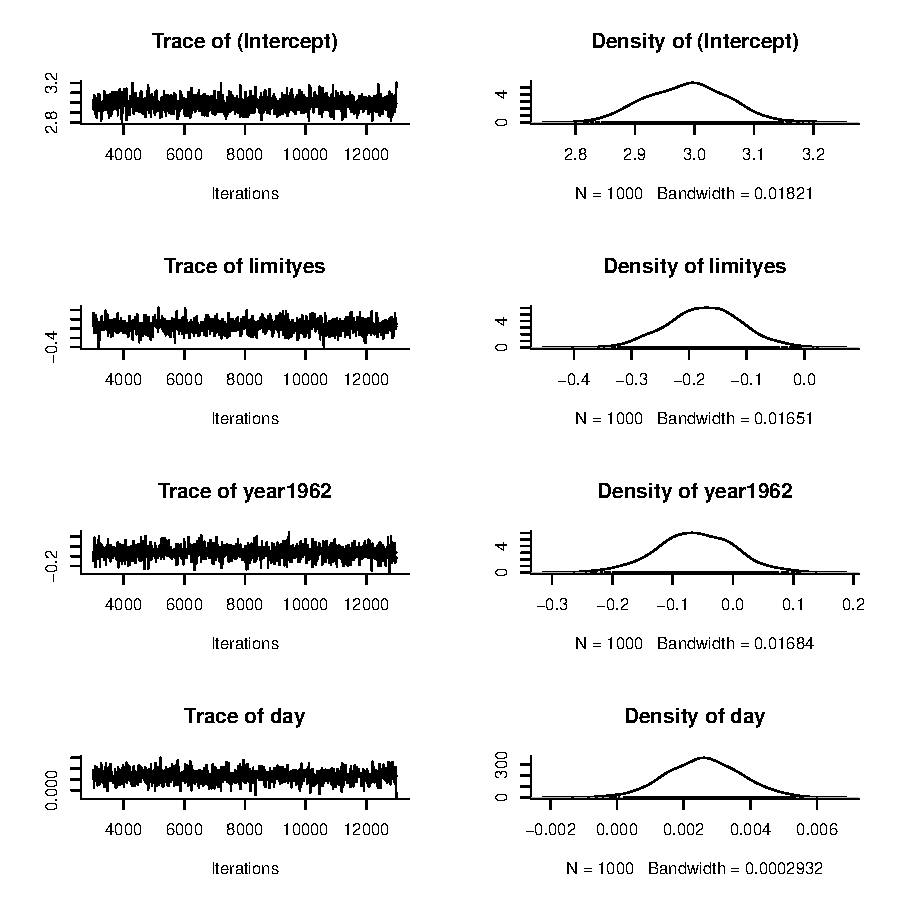
\includegraphics{Lecture2-019}
\end{center}
\caption{MCMC summary plot for the coefficients from a Poisson glm (model \texttt{m2a.5}).}
\label{mcmc.traffic-fig}
\end{figure}

Notice that the \texttt{year1962} coefficient has a high posterior density around zero, in agreement with the over-dispersed \texttt{glm} model, and that in general the estimates for the two models are broadly similar. This agreement is superficial.\\  

With additive over-dispersion the linear predictor includes a `residual', for which a residual variance is estimated (hence our prior specification). 

\begin{equation}
E[{\bf y}] = \textrm{exp}({\bf X}{\bm \beta}+{\bf e})
\end{equation}

At this point it will be handy to represent the linear model in a new way:

\begin{equation}
{\bf l} = {\bm \eta}+{\bf e}
\end{equation}

where ${\bf l}$ is a vector of latent variables ($\textrm{log}(E[{\bf y}])$ in this case) and eta (${\bm \eta}$) the usual symbol for the linear predictor (${\bf X}{\bm \beta}$). The data we observe are assumed to be Poisson variables with expectation equal to the exponentiated latent variables: 

\begin{equation}
{\bf y} \sim Pois(\textrm{exp}({\bf l}))
\end{equation}


Note that the latent variable does not exactly predict $y$, as it would if the data were Gaussian, because there is additional variability in the Poisson process. In the call to \texttt{MCMCglmm} I specified \texttt{pl=TRUE} to indicate that I wanted to store the posterior distributions of latent variables. This is not usually necessary and can require a lot of memory (we have 1000 realisations for each of the 182 data points). However as an example we can obtain the posterior mean residual for data point 92 which is the data from day 92 in 1961 when there was no speed limit:

\begin{Schunk}
\begin{Sinput}
> lat92 <- m2a.5$Liab[, 92]
> eta92 <- m2a.5$Sol[, "(Intercept)"] + m2a.5$Sol[, "day"] * Traffic$day[92]
> resid92 <- lat92 - eta92
> mean(resid92)
\end{Sinput}
\begin{Soutput}
[1] -0.1410748
\end{Soutput}
\end{Schunk}

This particular day has a negative expected residual indicating that the probability of getting injured was less than expected for this \emph{particular} realisation of that day in that year. If that \emph{particular} day could be repeated it does not necessarily mean that the actual number of injuries would always be less than expected, because it would follow a Poisson distribution with rate parameter $\lambda=$exp(\texttt{lat92})=21.872. In fact there would be a 21.461\% chance of having more injuries than if the residual had been zero:

\begin{Schunk}
\begin{Sinput}
> 1 - ppois(exp(mean(eta92)), exp(mean(lat92)))
\end{Sinput}
\begin{Soutput}
[1] 0.2146055
\end{Soutput}
\end{Schunk}

 Like residuals in a Gaussian model, the residuals are assumed to be independently and normally distributed with an expectation of zero and an estimated variance.  If the residual variance was zero then ${\bf e}$ would be a vector of zeros and the model would conform to the standard Poisson GLM. However, the posterior distribution of the residual variance is located well away form zero: 

\begin{Schunk}
\begin{Sinput}
> plot(m2a.5$VCV)
\end{Sinput}
\end{Schunk}

\begin{figure}[!h]
\begin{center}
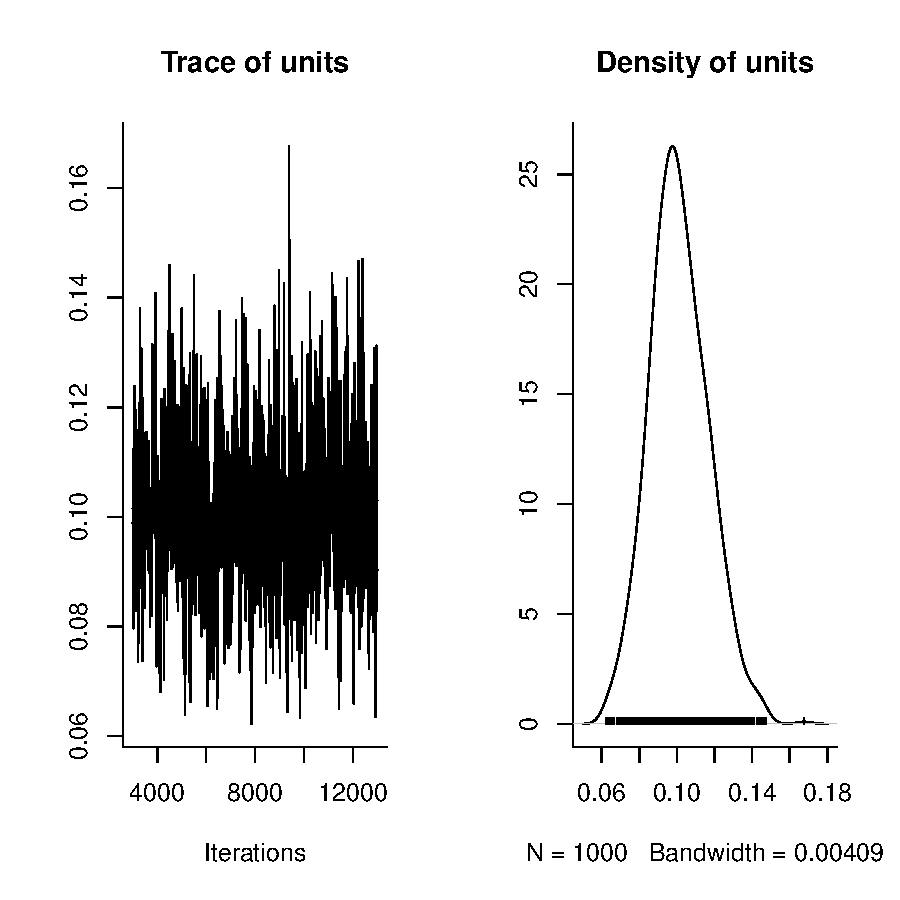
\includegraphics{Lecture2-023}
\end{center}
\caption{MCMC summary plot for the residual (\texttt{units})  variance from a Poisson glm (model \texttt{m2a.5}). The residual variance models any over-dispersion, and a residual variance of zero implies that the response conforms to a standard Poisson.}
\label{vcv.traffic-fig}
\end{figure}

The forces that created this residual were only realised on day 92 in 1961, however we could ask hypothetically what if those forces were present on another day. Figure \ref{prediction1-fig} plots the first 92 residuals as function of day (red lines) as scatter around the expectation on the log scale (solid black line). Each residual is only realised once, and the black dashed line is the hypothetical \texttt{resid92} which happened to be observed on day 92 (black circle).\\


\iftalk
\else
\fi

\iftalk
\else
\fi

\begin{figure}
\begin{minipage}[b]{0.5\linewidth} % A minipage that covers half the page
%\centering
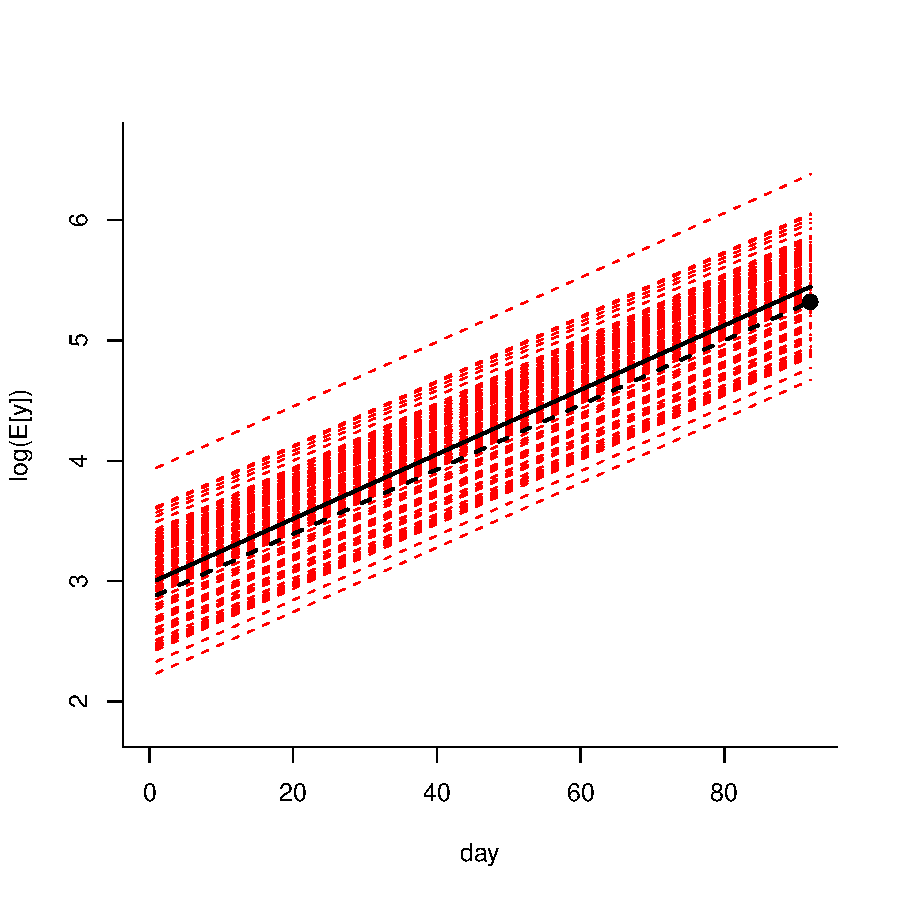
\includegraphics{Lecture2-029}
\end{minipage}
\hspace{0.2cm} % To get a little bit of space between the figures
\begin{minipage}[b]{0.5\linewidth}
%\centering
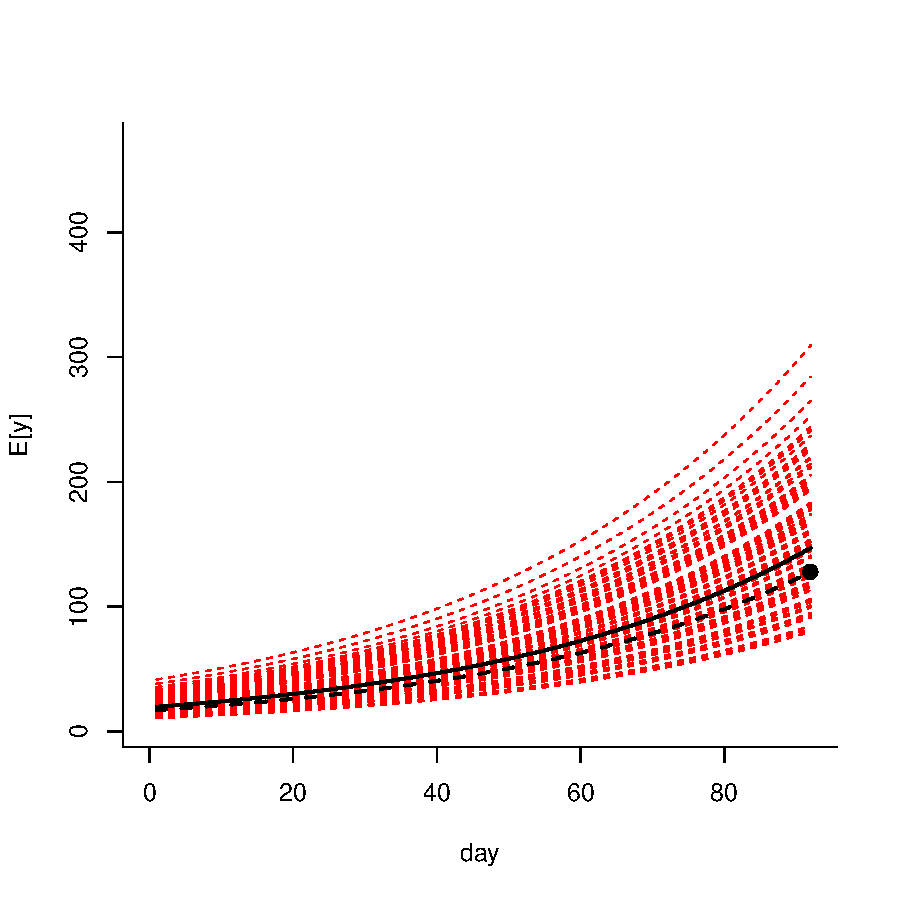
\includegraphics{Lecture2-030}
\end{minipage}
\caption{The predicted number of injuries on the log scale (left) and data scale (right) as a function of the continuous covariate \texttt{day} for 1961 without a speed limit. In order to highlight a point, the slope of the plotted relationship is an order of magnitude steeper than the model \texttt{m2a.5} estimate.  The solid black line is the value of the linear predictor, and the red dashed lines represent noise around the linear predictor. Each dashed line is a residual from the model, which is only observed for a particular data point. The vertical distance between the black dot and the solid black line is the observed residual on day 92. The black dashed line is the predicted value of a data point observed on other days but with the same residual value.  All lines are parallel and linear on the log scale, but this is not the case on the data scale.
}
\label{prediction1-fig}
\end{figure}


It is perhaps more interesting to know the expected number of injuries that would occur on this date if we had randomly sampled one of these other residuals. To indicate an expectation taken over residuals I have subscripted expectations with $e$.  In Figure \ref{prediction3-fig}  I have plotted the distribution of the latent variables on day 92. On the log scale the expectation is simply the solid black line $\eta$. However, because the exponent function is non-linear this does not translate to the data scale and $\eta$ is actually equal to the median value on the data scale.\\ 


\iftalk
\else
\fi

\iftalk
\else
\fi

\begin{figure}
\begin{minipage}[b]{0.5\linewidth} % A minipage that covers half the page
\centering
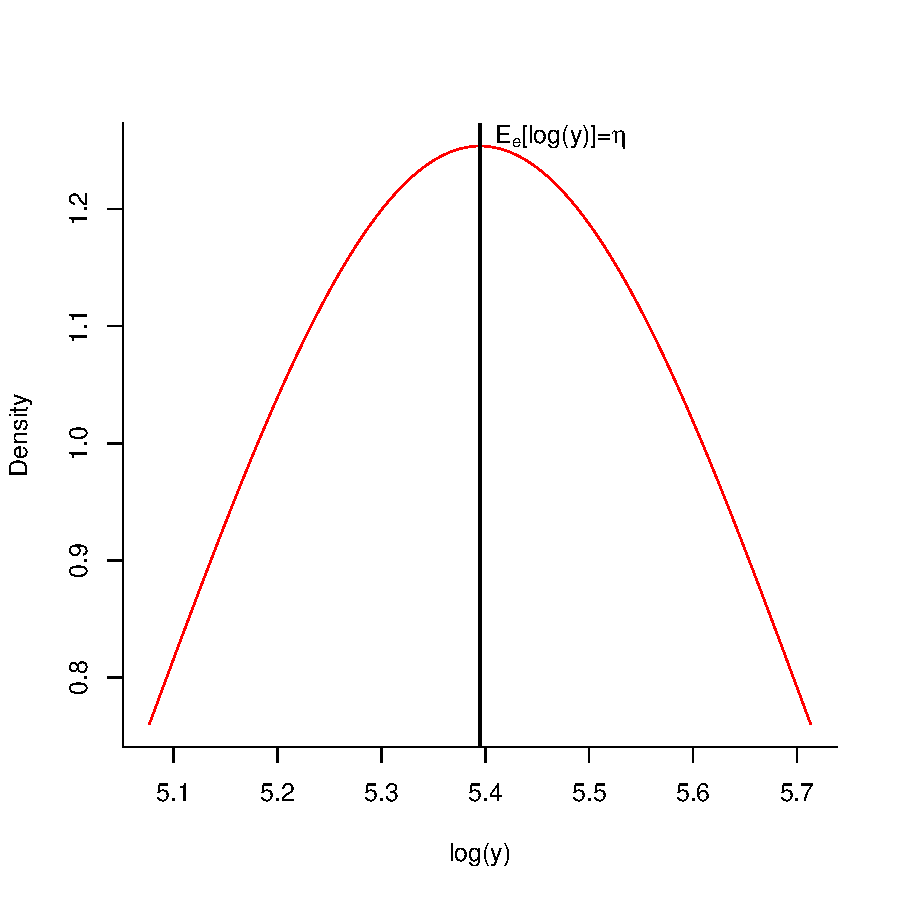
\includegraphics{Lecture2-037}
\end{minipage}
\hspace{0.5cm} % To get a little bit of space between the figures
\begin{minipage}[b]{0.5\linewidth}
\centering
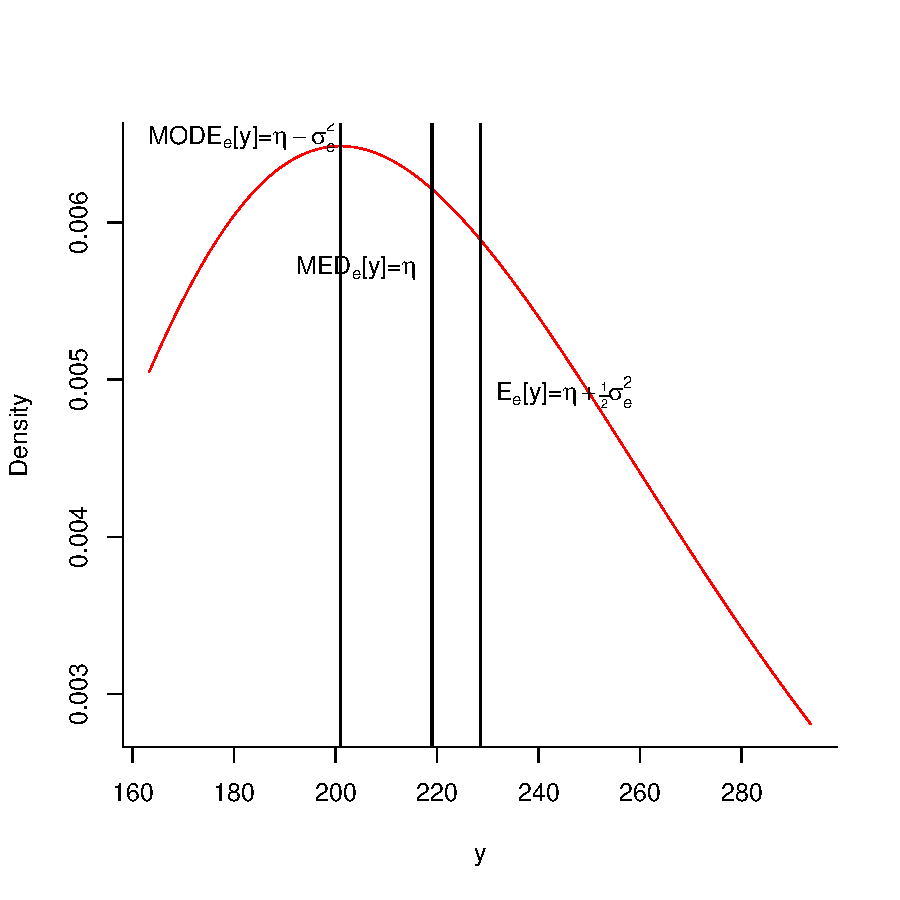
\includegraphics{Lecture2-038}
\end{minipage}
\caption{The hypothetical distribution for the number of injuries on the log scale (left) and data scale (right) for day 92 in 1961 without a speed limit. These can viewed as vertical slices from Figure \ref{prediction1-fig} on day 92. On the log scale the distribution is assumed to be normal and so the residuals are symmetrically distributed around the linear predictor. As a consequence the linear predictor ($\eta$) is equal to the mean, median and mode of the distribution on the log scale. Because the exponential function is non-linear this symmetry is lost on the data scale, and the different measures of central tendency do not coincide. Since the residuals are normal on the log scale, the distribution on the data scale is log-normal and so analytical solutions exist for the mean, mode and median.  $\sigma^{2}$ is the residual variance.
}
\label{prediction3-fig}
\end{figure}

In the \texttt{Traffic} example the non linearities are small so the differences in parameter estimates are not large using either multiplicative or additive models. However, multiplying the intercept in model \texttt{m2a.5} by half the residual variance is in closer agreement with the quasipoisson model than the raw intercept:

\begin{Schunk}
\begin{Sinput}
> exp(mean(m2a.5$Sol[, "(Intercept)"] + 0.5 * m2a.5$VCV[, 1]))
\end{Sinput}
\begin{Soutput}
[1] 20.91752
\end{Soutput}
\begin{Sinput}
> exp(mean(m2a.5$Sol[, "(Intercept)"]))
\end{Sinput}
\begin{Soutput}
[1] 19.88554
\end{Soutput}
\begin{Sinput}
> exp(m2a.3$coef["(Intercept)"])
\end{Sinput}
\begin{Soutput}
(Intercept) 
   21.54891 
\end{Soutput}
\end{Schunk}

Analytical results for these transformations can be obtained for the Poisson log-normal, but for other distributions this is not always the case. Section \ref{pred-sec} gives prediction functions for other types of distribution. One could reasonably ask, why have this additional layer of complexity, why not just stick with the multiplicative model? This brings us to random effects. 


\section{Random effects}
\label{ranef-sec}

In some cases we may have measured variables whose effects we would like to treat as random. Often the distinction between fixed and random is given by example; things like population, species, individual and vial are random, but sex, treatment and age are not. Or the distinction is made using rules of thumb; if there are few factor levels and they are interesting to other people they are fixed.  However, this doesn't really confer any understanding about what it means to treat something as fixed or random, and doesn't really allow judgements to be made regarding ambiguous variables (for example year) or give any insight into the fact that in a Bayesian analysis all effects are technically random.\\

When we treat an effect as fixed we believe that the only information regarding its value comes from data associated with that particular level. If we treat  an effect as random we also use this information, but we weight it by what other data tell us about the likely values that the effects could take. In a Bayesian analysis this additional information could come from data not formally included in the analysis, in which case it would be called a prior. In hierarchical models this additional information comes from data associated with other factor levels of the same type.\\

The degree to which this additional information is important depends on the variability of the effects, as measured by the estimated variance component, and the degree of replication within a particular level. If variability is high then most of the information must come from data associated with an individual effect, particularly if replication within that effect is high. However, if variability and replication are low then extreme mean values of the response for a given level are more likely to be due to sampling error alone, and so the estimates are shrunk towards zero.\\

It is common to hear things like `year is a random effect' as if you just have to estimate \emph{a} single effect for all years. It is also common to hear things like `years is random' as if years were sampled at random.  Better to say year effects are random and understand that it is the effects that are random not the years, and that we're trying to estimate as many effects as there are years.  In this sense they're the same as fixed effects, and we can easily treat the year effects as random to see what difference it makes.\\ 

Random effect models are often expressed as:

\begin{equation}
E[{\bf y}] = \textrm{exp}({\bf X}{\bm \beta}+{\bf Z}{\bf u}+{\bf e})
\end{equation}

where ${\bf Z}$ is a design matrix like ${\bf X}$, and ${\bf u}$ is a vector of parameters like ${\bm \beta}$. We can specify simple random effect models in the same way that we specified the fixed effects:

\begin{Schunk}
\begin{Soutput}
random =  ~ year
\end{Soutput}
\end{Schunk}

although we don't need anything to the left of the $\sim$ because the response is known from the fixed effect specification. In addition, the global intercept is suppressed by default, so in fact this specification produces the design matrix:

\begin{Schunk}
\begin{Sinput}
> Z <- model.matrix(~year - 1, data = Traffic)
> Z[c(1, 2, 184), ]
\end{Sinput}
\begin{Soutput}
    year1961 year1962
1          1        0
2          1        0
184        0        1
\end{Soutput}
\end{Schunk}

Earlier I said that there was no distinction between fixed and random effects in a Bayesian analysis - all effects are random - so lets not make the distinction and combine the design matrices (${\bf W} = [{\bf X}, {\bf Z}]$) and combine the vectors of parameters (${\bm \theta} = [{\bm \beta}^{'}, {\bf u}^{'}]^{'}$):

\begin{equation}
E[{\bf y}] = \textrm{exp}({\bf W}{\bm \theta}+{\bf e})
\label{MM-eq}
\end{equation}

If we drop year from the fixed terms, the new fixed effect design matrix looks like:

\begin{Schunk}
\begin{Sinput}
> X2 <- model.matrix(y ~ limit + day, data = Traffic)
> X2[c(1, 2, 184), ]
\end{Sinput}
\begin{Soutput}
    (Intercept) limityes day
1             1        0   1
2             1        0   2
184           1        1  92
\end{Soutput}
\end{Schunk}

and

\begin{Schunk}
\begin{Sinput}
> W <- cbind(X2, Z)
> W[c(1, 2, 184), ]
\end{Sinput}
\begin{Soutput}
    (Intercept) limityes day year1961 year1962
1             1        0   1        1        0
2             1        0   2        1        0
184           1        1  92        0        1
\end{Soutput}
\end{Schunk}

You will notice that this new design matrix is  exactly equivalent to the original design matrix \texttt{X} except we have one additional variable \texttt{year1961}. In our first model this variable was absorbed in to the global intercept because it could no be uniquely estimated from the data. What has changed that could make this additional parameter estimable?  As is usual in a Bayesian analysis, if there is no information in the data it has to come from the prior. In model \texttt{m2a.5} we used the default normal prior for the fixed effects with means of zero, large variances of $10^{8}$, and no covariances. Lets treat the year effects as random, but rather than estimate a variance component for them we'll fix the variance  at $10^{8}$ in the prior:

\begin{Schunk}
\begin{Sinput}
> prior <- list(R = list(V = 1, nu = 0.002), G = list(G1 = list(V = 1e+08, 
+     fix = 1)))
> m2a.6 <- MCMCglmm(y ~ limit + day, random = ~year, family = "poisson", 
+     data = Traffic, prior = prior, verbose = FALSE, pr = TRUE)
> plot(m2a.6$Sol)
\end{Sinput}
\end{Schunk}




\begin{figure}[!h]
\begin{center}
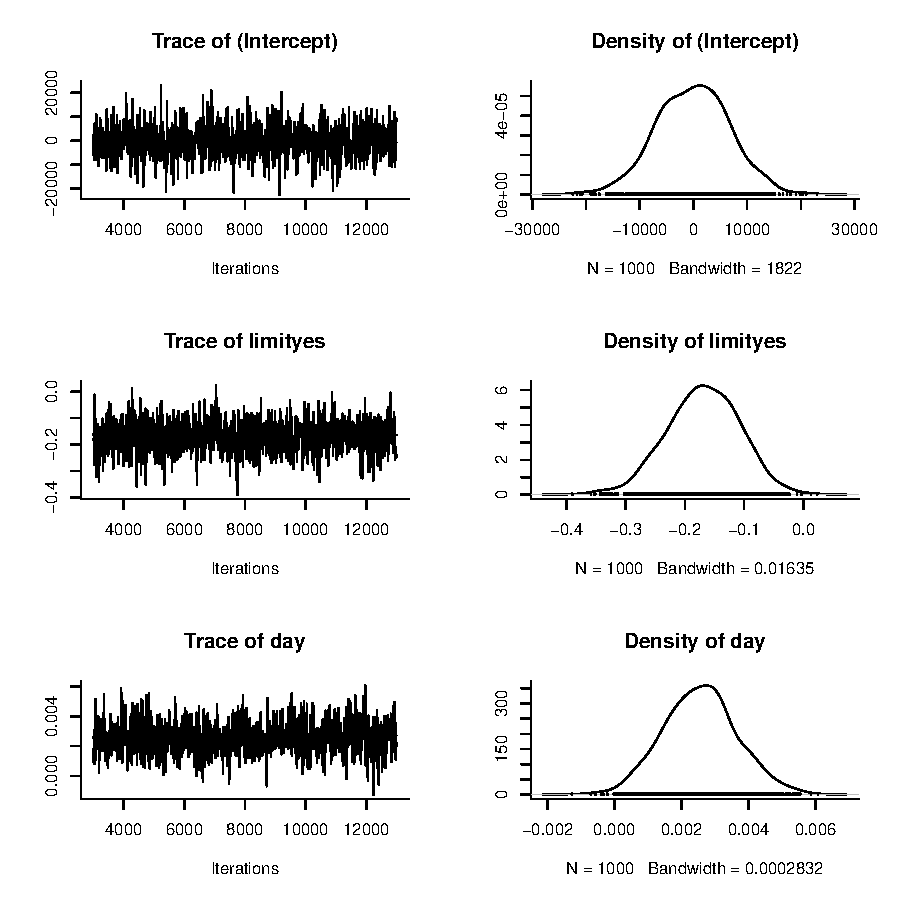
\includegraphics{Lecture2-046}
\end{center}
\caption{MCMC summary plots for the intercept, speed limit and day coefficients from model \texttt{m2a.6} where year effects were treated as random. Note the high posterior variance for the intercept.}
\label{yrandom-fig}
\end{figure}

The estimates for the intercept, day and the effect of a speed limit now appear completely different (Figure \ref{yrandom-fig}).  However, in the original model (\texttt{m2a.5}) the prediction for each year is obtained by:

\begin{Schunk}
\begin{Sinput}
> y1961.m2a.5 <- m2a.5$Sol[, "(Intercept)"]
> y1962.m2a.5 <- m2a.5$Sol[, "(Intercept)"] + m2a.5$Sol[, "year1962"]
\end{Sinput}
\end{Schunk}

However, for this model we have to add the intercept to both random effects to get the year predictions. \texttt{MCMCglmm} does not store the posterior distribution of the random effects by default, but because we specified \texttt{pr=TRUE}, the whole of ${\bm \theta}$ is stored rather than just ${\bm \beta}$:  

\begin{Schunk}
\begin{Sinput}
> y1961.m2a.6 <- m2a.6$Sol[, "(Intercept)"] + m2a.6$Sol[, "year.1961"]
> y1962.m2a.6 <- m2a.6$Sol[, "(Intercept)"] + m2a.6$Sol[, "year.1962"]
\end{Sinput}
\end{Schunk}

We can merge the two posterior distributions to see how they compare:

\begin{Schunk}
\begin{Sinput}
> y.m2a.5 <- mcmc(cbind(y1961 = y1961.m2a.5, y1962 = y1962.m2a.5))
> y.m2a.6 <- mcmc(cbind(y1961 = y1961.m2a.6, y1962 = y1962.m2a.6))
> plot(mcmc.list(y.m2a.5, y.m2a.6))
\end{Sinput}
\end{Schunk}


\begin{figure}[!h]
\begin{center}
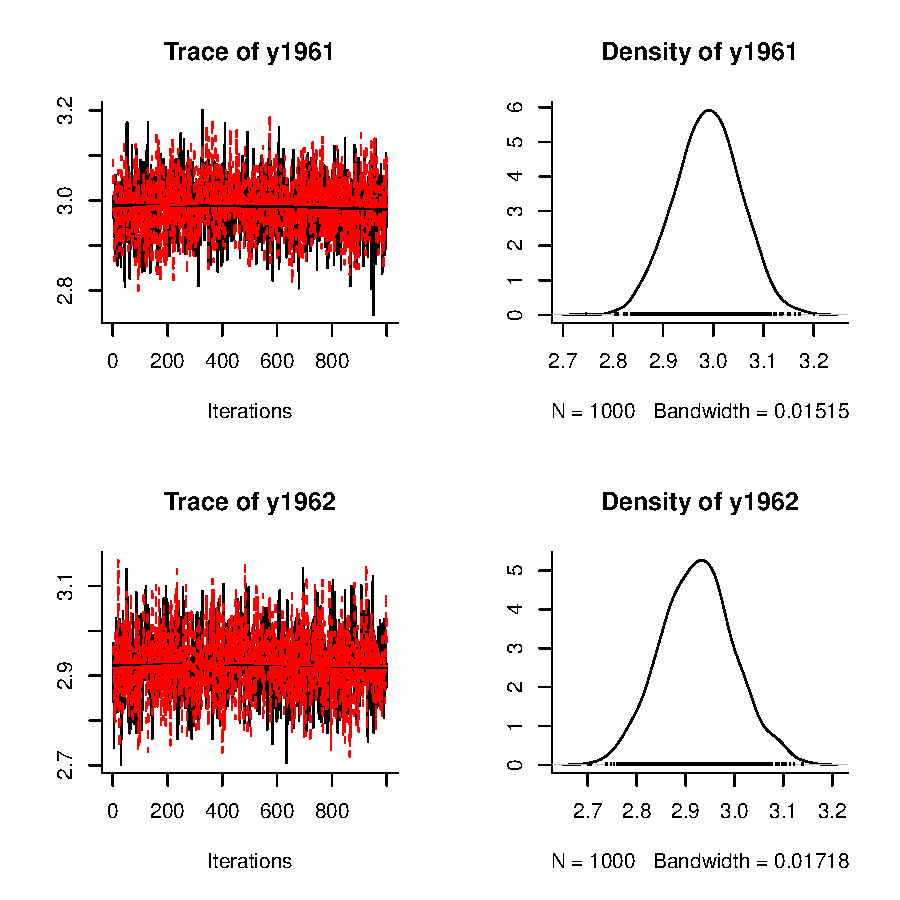
\includegraphics{Lecture2-050}
\end{center}
\caption{MCMC summary plots for the year effects from a model where year effects were treated as fixed (black) and where they were treated as random (red) but with the variance component set at a large value rather than being estimated. The posterior distributions are virtually identical.}
\label{y.pred-fig}
\end{figure}

The posterior distributions are very similar (Figure \ref{y.pred-fig}; but see Section \ref{PriorContr-sec} why they are not identical), highlighting the fact that effects that are fixed are those associated with a variance component which has been set \emph{a priori} to something large ($10^8$ in this case), where effects that are random are associated with a variance component which is not set \emph{a priori} but is estimated from the data. As the variance component tends to zero then no matter how many random effects there are, we are effectively only estimating a single parameter (the variance). This makes sense, if there were no differences between years we only need to estimate a global intercept and not separate effects for each year. Alternatively if the variance is infinite then we need to estimate separate effects for each year. In this case the intercept is confounded with the average value of the random effect, resulting in a wide marginal distribution for the intercept, and strong posterior correlations between the intercept and the mean of the random effects:

\begin{Schunk}
\begin{Sinput}
> plot(c(m2a.6$Sol[, "year.1961"] + m2a.6$Sol[, "year.1962"])/2, 
+     c(m2a.6$Sol[, "(Intercept)"]))
\end{Sinput}
\end{Schunk}


\begin{figure}[!h]
\begin{center}
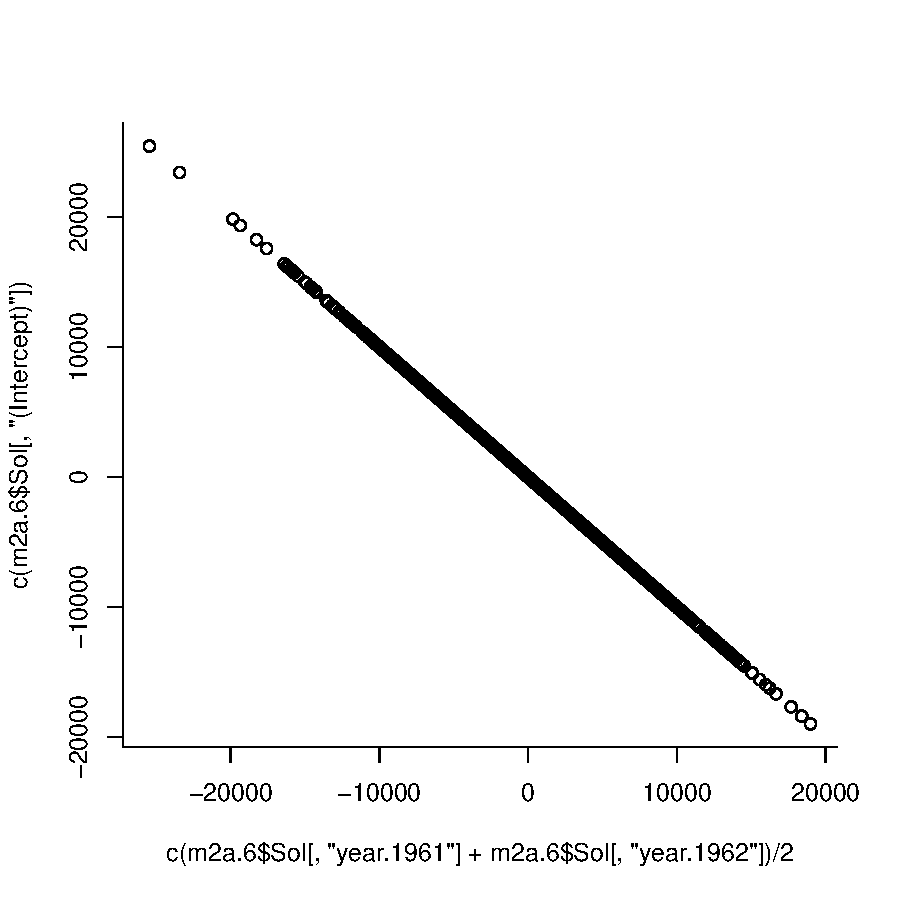
\includegraphics{Lecture2-052}
\end{center}
\caption{Joint posterior distribution of the intercept and the mean of the two random year effects. The variance component associated with year was fixed at a large value ($10^8$) and so the effects are almost completely confounded.}
\label{yfixed-fig}
\end{figure}

With only two levels, there is very little information to estimate the variance, and so we would often make the \emph{a priori} decision to treat year effects as fixed, and fix the variance components to something large (or infinity in a frequentist analysis).\\

At the moment we have day as a continuous covariate, but we could also have random day effects and ask whether the number of injuries on the same day but in different years are correlated. Rather than fixing the variance component at something large, we'll use the same weaker prior that we used for the residual variance:

\begin{Schunk}
\begin{Sinput}
> Traffic$day <- as.factor(Traffic$day)
> prior <- list(R = list(V = 1, nu = 0.002), G = list(G1 = list(V = 1, 
+     nu = 0.002)))
> m2a.7 <- MCMCglmm(y ~ year + limit + as.numeric(day), random = ~day, 
+     family = "poisson", data = Traffic, prior = prior, verbose = FALSE)
\end{Sinput}
\end{Schunk}

\texttt{day} has also gone in the fixed formula, but as a numeric variable, in order to capture any time trends in the number of injuries. Most of the over-dispersion seems to be captured by fitting day as a random term (Figure \ref{GLMM.VCV-fig}):

\begin{Schunk}
\begin{Sinput}
> plot(m2a.7$VCV)
\end{Sinput}
\end{Schunk}

\begin{figure}[!h]
\begin{center}
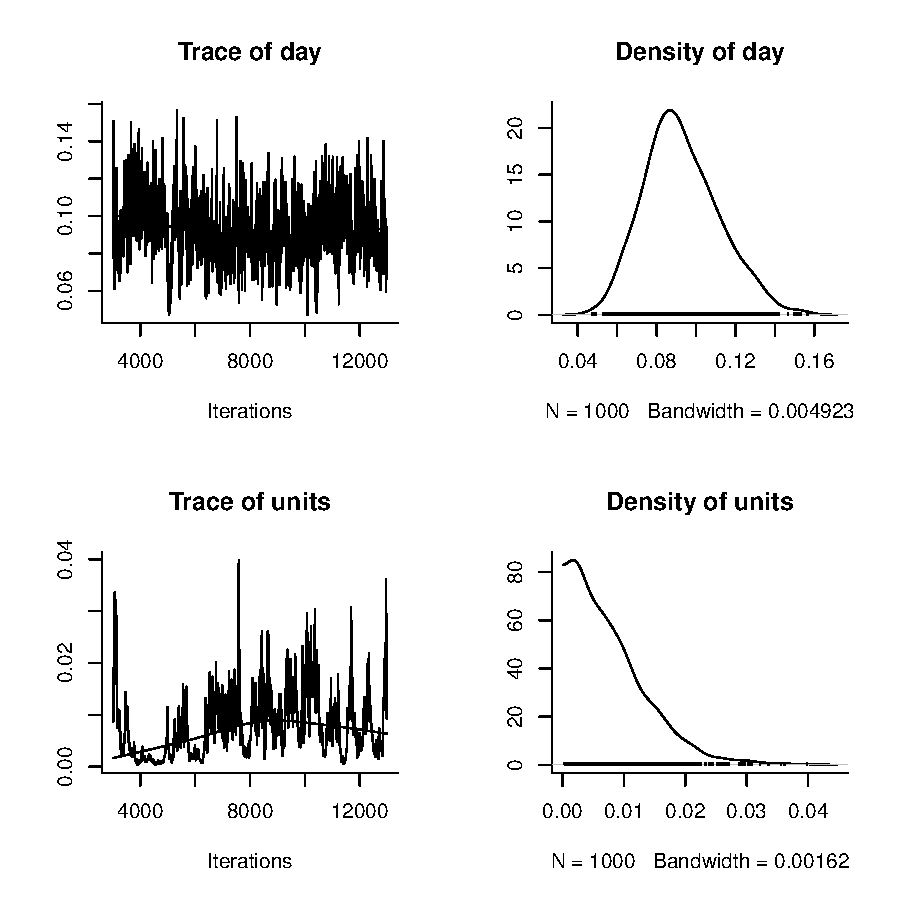
\includegraphics{Lecture2-055}
\end{center}
\caption{MCMC summary plot of the variance component associated with day (top) and the residual variance component (below). The trace for the residual variance shows strong autocorrelation and needs to be ran for longer.}
\label{GLMM.VCV-fig}
\end{figure}

In fact it explains so much that the residual variance is close to zero and mixing seems to be a problem. The chain would have to be run for longer, and the perhaps an alternative prior specification used.

\section{Prediction with Random effects}
\label{pred-sec}

In section \ref{addod-sec} we showed that for non-Gaussian data the expectation of the response variable $y$ is different from the linear predictor if we wish to average over the residuals. Often it is important to get the expectation after marginalising residuals, and indeed after marginalising other random effects. For example we may not be so interested in knowing the expected number of injuries on the average day, but knowing the expected number of injuries on any random day. \\  

For the Poisson mixed model:

\begin{equation}
E[y] = \texttt{exp}({\bf X}{\bm \beta}+{\bf Z}{\bf u}+{\bf e})
\end{equation}

we can marginalise with respect to the random effects, including the over-dispersion residual:

\begin{equation}
E_{{u,e}}[y] = \textrm{exp}({\bf X}{\bm \beta}+0.5\sigma^{2})
\end{equation}

where $\sigma^{2}$ is the sum of the variance components.\\

For the Binomial mixed model with logit link

\begin{equation}
E[y] = \textrm{logit}^{-1}({\bf X}{\bm \beta}+{\bf Z}{\bf u}+{\bf e})
\end{equation}

it is not possible to marginilse with respect to the random effects analytically, but two approximations exist. The first

\begin{equation}
E_{{u,e}}[y] \approx \textrm{logit}^{-1}({\bf X}{\bm \beta}-0.5\sigma^{2}\textrm{tanh}({\bf X}{\bm \beta}(1+2\textrm{exp}(-0.5\sigma^{2}))/6)))
\end{equation}

can be found on p452 in \citet{McCulloch.2001} and the second (and possibly less accurate) approximation in \citet{Diggle.2004}:


\begin{equation}
E_{{u,e}}[y] \approx \textrm{logit}^{-1}\left(\frac{{\bf X}{\bm \beta}}{\sqrt{1+(\frac{16\sqrt{3}}{15\pi})^{2}\sigma^{2}}}\right)
\end{equation}



A predict function has been implemented for \texttt{MCMCglmm} although it is currently incomplete and needs further testing. However, for simpler distributions it should be OK - for example, we can predict the laibality on the latent scale after marginalising the random effects in model \texttt{m2a.7}:

\begin{Schunk}
\begin{Sinput}
> predict(m2a.7, marginal = ~day, type = "terms")[1:5]
\end{Sinput}
\begin{Soutput}
[1] 3.013906 3.016406 3.018907 3.021407 3.023907
\end{Soutput}
\end{Schunk}

or we can predict on the data scale:

\begin{Schunk}
\begin{Sinput}
> predict(m2a.7, marginal = ~day, type = "response")[1:5]
\end{Sinput}
\begin{Soutput}
[1] 22.41390 22.46803 22.52232 22.57679 22.63144
\end{Soutput}
\end{Schunk}

In addition, credible intervals can be obtained 

\begin{Schunk}
\begin{Sinput}
> predict(m2a.7, marginal = ~day, type = "response", interval = "confidence")[1:5, 
+     ]
\end{Sinput}
\begin{Soutput}
       fit      lwr      upr
1 22.41390 19.19317 25.93465
2 22.46803 19.28033 25.94429
3 22.52232 19.36215 25.95811
4 22.57679 19.39551 25.93856
5 22.63144 19.47556 25.93655
\end{Soutput}
\end{Schunk}

as can prediction intervals through posterior predictive simulation:

\begin{Schunk}
\begin{Sinput}
> predict(m2a.7, marginal = ~day, type = "response", interval = "prediction")[1:5, 
+     ]
\end{Sinput}
\begin{Soutput}
       fit      lwr      upr
1 22.14200 7.307660 44.72613
2 22.13422 5.424454 41.50115
3 22.36608 6.893520 41.15897
4 22.14274 6.968208 42.67847
5 22.27424 6.286758 40.72599
\end{Soutput}
\end{Schunk}

\section{Categorical Data}

Response variables consisting of levels of some categorical factor are best analysed using \texttt{family="categorical"} if the levels have no natural ordering,  or \texttt{family="ordinal"} if the levels do have a natural ordering, such as never $<$ sometimes $<$ always. The simplest variable of this type is binary data where the response variable is either a zero or a one, and can be analysed as \texttt{family="categorical"} (logit link) or \texttt{family="ordinal"} (probit link).   A binary distribution is a special case of the binomial distribution where the number of trials (\texttt{size}) is equal to 1. One way of interpreting a binomial response is to expand it into a series of binary variables and treat the zero's and ones as repeated measures. For example, we could generate two binomial variates each with 5 trials:

\begin{Schunk}
\begin{Sinput}
> success <- rbinom(2, size = 5, prob = c(0.4, 0.6))
> failure <- 5 - success
> binom <- rbind(success, failure)
> colnames(binom) <- c("u.1", "u.2")
> binom
\end{Sinput}
\begin{Soutput}
        u.1 u.2
success   3   3
failure   2   2
\end{Soutput}
\end{Schunk}

and then expand them into success or failure:

\begin{Schunk}
\begin{Sinput}
> binary <- matrix(rep(c(1, 0, 1, 0), binom), 1, 10)
> colnames(binary) <- rep(c("u.1", "u.2"), each = 5)
> binary
\end{Sinput}
\begin{Soutput}
     u.1 u.1 u.1 u.1 u.1 u.2 u.2 u.2 u.2 u.2
[1,]   1   1   1   0   0   1   1   1   0   0
\end{Soutput}
\end{Schunk}

We can then interpret the \texttt{units} variance in a binomial GLMM as accounting for any similarity between repeated measurements made within the same observational unit. If the binary variables within the binomial observation are correlated, this means that the underlying probability for each binomial response differs to a greater degree than can be predicted from the linear predictor. In this example the two probabilities were 0.4 and 0.6 which means that the repeated binary measures would be correlated if we only fitted the intercept (0.5).\\  

If the original data are already binary then there is no information to measure how repeatable trials are within a binomial unit because we only have a single trial per observation. This does not necessarily mean that heterogeneity in the underlying probabilities does not exist, only that we can't estimate it. Imagine we are in a room of 100 people and we are told that 5\% of the people will be dead the following day.  If the people in the room were a random sample from the UK population I would worry - \emph{I} probably have a 5\% chance of dying. If on the other hand the room was a hospital ward and I was a visitor, I may not worry too much for \emph{my} safety. The point is that in the absence of information, the binary data look the same if each person has a 5\% chance of dying or if 5 people have a 100\% chance of dying.  Most programs set the residual variance to zero and assume the former, but it is important to understand that this is a convenient but arbitrary choice. Given this, it is desirable that any conclusions drawn from the model do not depend on this arbitrary choice. Worryingly, both the location effects (fixed and random) and variance components are completely dependent on the magnitude of the residual variance.\\

To demonstrate we will use some data from a pilot study on the Indian meal moth (\emph{Plodia interpunctella}) and its granulosis virus (PiGV) collected by Hannah Tidbury \& Mike Boots at the University of Sheffield.

\begin{Schunk}
\begin{Sinput}
> data(PlodiaRB)
\end{Sinput}
\end{Schunk}

The data are taken from  874 moth pupae for which the \texttt{Pupated} variable is zero if they failed to pupate (because they were infected with the virus) or one if they successfully pupated. The 874 individuals are spread across 49 full-sib families, with family sizes ranging from 6 to 38.\\

To start we will fix the residual variance at 1:

\begin{Schunk}
\begin{Sinput}
> prior.m2b.1 = list(R = list(V = 1, fix = 1), G = list(G1 = list(V = 1, 
+     nu = 0.002)))
> m2b.1 <- MCMCglmm(Pupated ~ 1, random = ~FSfamily, family = "categorical", 
+     data = PlodiaRB, prior = prior.m2b.1, verbose = FALSE)
\end{Sinput}
\end{Schunk}

and then fit a second model where the residual variance is fixed at 2:

\begin{Schunk}
\begin{Sinput}
> prior.m2b.2 = list(R = list(V = 2, fix = 1), G = list(G1 = list(V = 1, 
+     nu = 0.002)))
> m2b.2 <- MCMCglmm(Pupated ~ 1, random = ~FSfamily, family = "categorical", 
+     data = PlodiaRB, prior = prior.m2b.2, verbose = FALSE)
\end{Sinput}
\end{Schunk}

The posterior distribution for the intercept differs between the two models (see Figure \ref{Bin1-fig}): 

\begin{Schunk}
\begin{Sinput}
> plot(mcmc.list(m2b.1$Sol, m2b.2$Sol))
\end{Sinput}
\end{Schunk}

\begin{figure}[!h]
\begin{center}
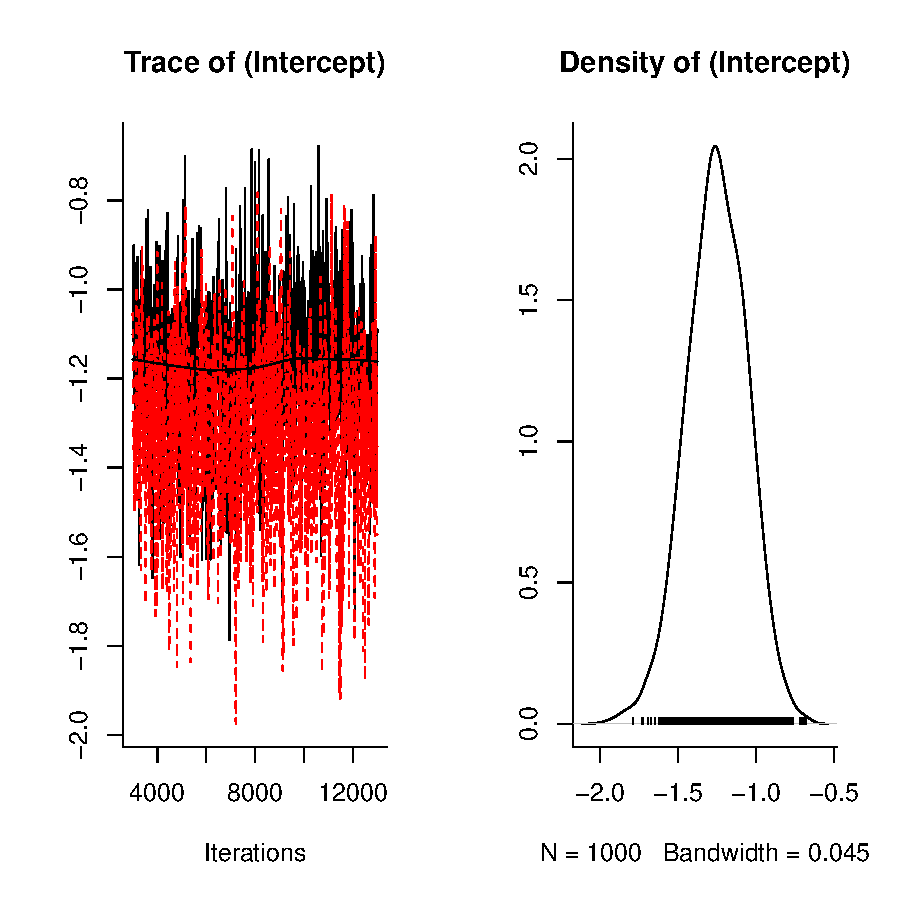
\includegraphics{Lecture2-066}
\end{center}
\caption{MCMC summary plots for the intercept of a binary GLMM where the residual variance was fixed at one (black) and two (red).}
\label{Bin1-fig}
\end{figure}

as do the variance components  (see Figure \ref{Bin2-fig}):

\begin{Schunk}
\begin{Sinput}
> plot(mcmc.list(m2b.1$VCV, m2b.2$VCV))
\end{Sinput}
\end{Schunk}

\begin{figure}[!h]
\begin{center}
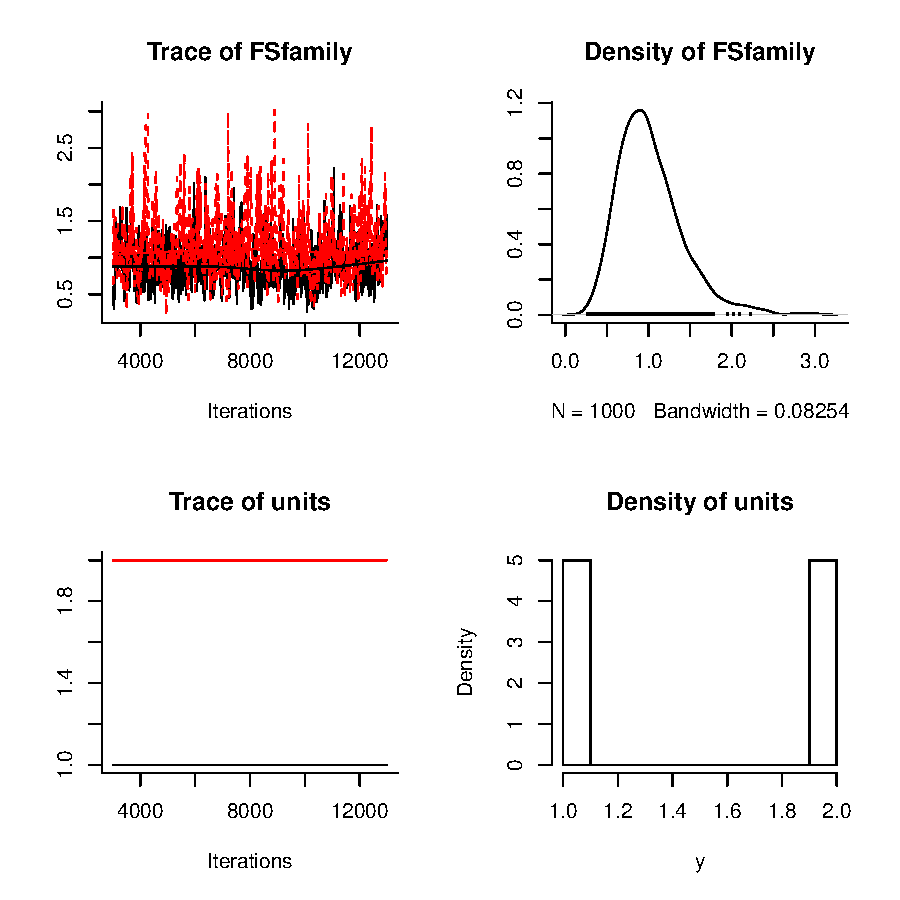
\includegraphics{Lecture2-068}
\end{center}
\caption{MCMC summary plots for the between family variance component of a binary GLMM where the residual variance was fixed at one (black) and two (red).}
\label{Bin2-fig}
\end{figure}

Should we worry? Not really. We just have to be careful about how we express the results. Stating that the family variance is 0.655 is meaningless without putting it in the context of the assumed residual variance. It is therefore more appropriate to report the intraclass correlation which in this context is the expected correlation between the state Pupated/Not Pupated, for members of the same family. It can be calculated as:

\begin{equation}
\texttt{IC} =  \frac{\sigma^{2}_{\texttt{FSfamily}}}{\sigma^{2}_{\texttt{FSfamily}}+\sigma^{2}_{\texttt{units}}+\pi^{2}/3} 
\end{equation} 

for the logit link, which is used when \texttt{family=categorical}, or 

\begin{equation}
\texttt{IC} =  \frac{\sigma^{2}_{\texttt{FSfamily}}}{\sigma^{2}_{\texttt{FSfamily}}+\sigma^{2}_{\texttt{units}}+1} 
\end{equation} 

for the probit link, which is used if \texttt{family=ordinal} was specified.\\

Obtaing the posterior distribution of the intra-calss correlation for each model shows that they are sampling very similar posterior distributions (see Figure \ref{IC-fig}) 

\begin{Schunk}
\begin{Sinput}
> IC.1 <- m2b.1$VCV[, 1]/(rowSums(m2b.1$VCV) + pi^2/3)
> IC.2 <- m2b.2$VCV[, 1]/(rowSums(m2b.2$VCV) + pi^2/3)
> plot(mcmc.list(IC.1, IC.2))
\end{Sinput}
\end{Schunk}

\begin{figure}[!h]
\begin{center}
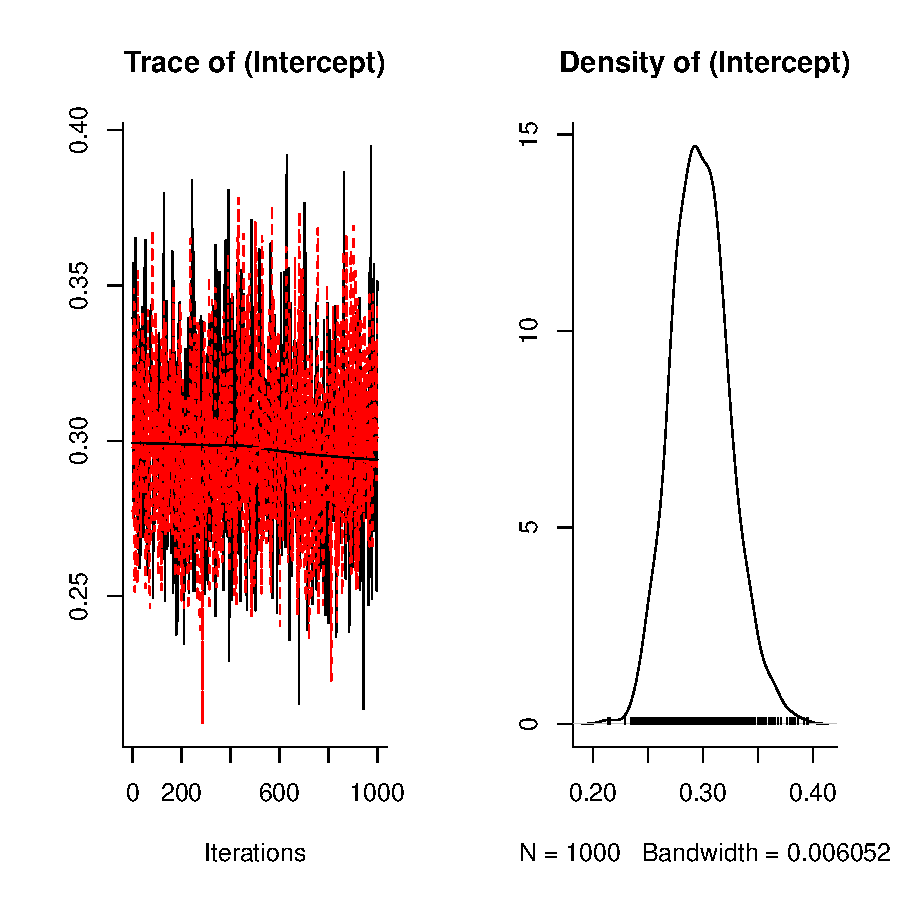
\includegraphics{Lecture2-070}
\end{center}
\caption{MCMC summary plots for the intra-family correlation from  a binary GLMM where the residual variance was fixed at one (black) and two (red).}
\label{IC-fig}
\end{figure}

Using the approximation due to \citet{Diggle.2004} described earlier we can also rescale the estimates by the estimated residual variance ($\sigma^{2}_{\texttt{units}}$) in order to obtain the posterior distributions of the parameters under the assumption that the actual residual variance ($\sigma^{2}_{e}$) is equal to some other value.  For location effects the posterior distribution needs to be multiplied by $\sqrt{\frac{1+c^{2}\sigma^{2}_{e}}{1+c^{2}\sigma^{2}_{\texttt{units}}}}$ and for the variance components the posterior distribution needs to be multiplied by $\frac{1+c^{2}\sigma^{2}_{e}}{1+c^{2}\sigma^{2}_{\texttt{units}}}$ where $c$ is some constant that depends on the link function. For the probit $c=1$ and for the logit $c=16\sqrt{3}/15\pi$. We can obtain estimates under the assumption that $\sigma^{2}_{e}=0$: 

\begin{Schunk}
\begin{Sinput}
> c2 <- ((16 * sqrt(3))/(15 * pi))^2
> Int.1 <- m2b.1$Sol/sqrt(1 + c2 * m2b.1$VCV[, 2])
> Int.2 <- m2b.2$Sol/sqrt(1 + c2 * m2b.2$VCV[, 2])
> plot(mcmc.list(as.mcmc(Int.1), as.mcmc(Int.2)))
\end{Sinput}
\end{Schunk}

\begin{figure}[!h]
\begin{center}
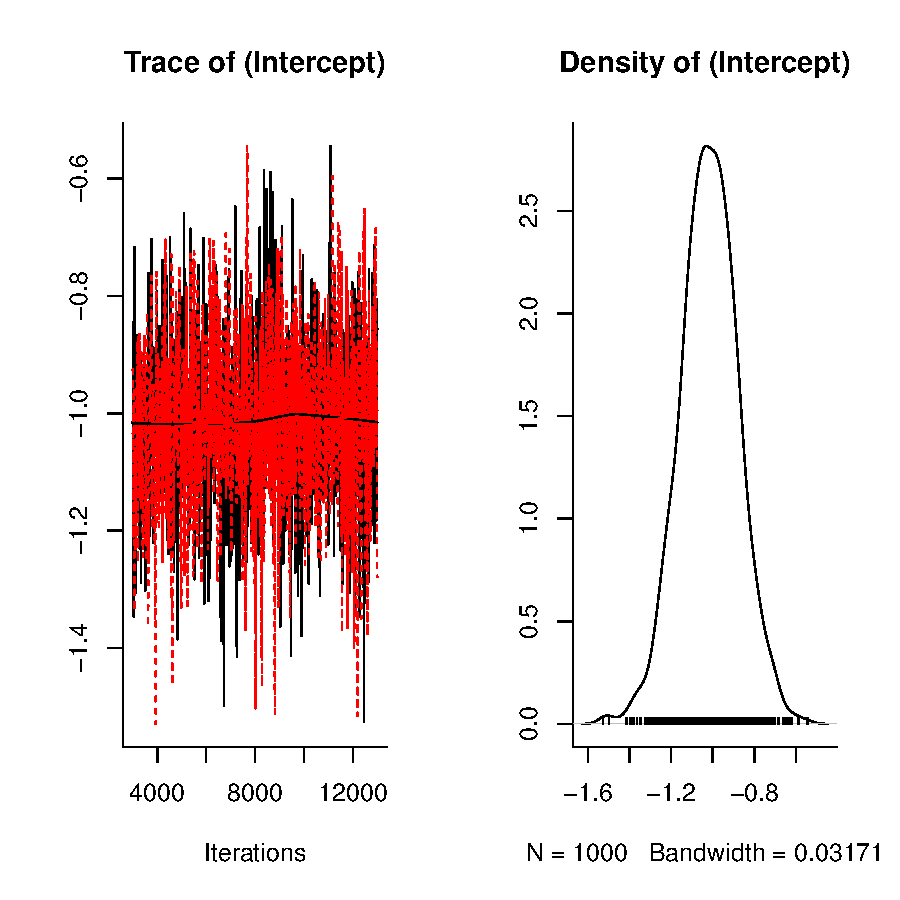
\includegraphics{Lecture2-072}
\end{center}
\caption{MCMC summary plots for the expected proportion of caterpillars pupating from  a binary GLMM where the residual variance was fixed at one (black) and two (red).}
\label{ICI-fig}
\end{figure}

The posteriors should be virtually identical under a flat prior (See Figure \ref{ICI-fig}) although with different priors this is not always the case. Remarkably, \citet{vanDyk.2001} show that leaving a diffuse prior on $\sigma^{2}_{\texttt{units}}$ and rescaling the estimates each iteration, a Markov chain with superior mixing and convergence properties can be obtained (See section \ref{secPX}).\\  

It should also be noted that a diffuse prior on the logit scale is not necessarily weakly informative on the probability scale. For example, the default setting for the prior on the intercept is $N(0, 10^{8})$ on the logit scale, which although relatively flat across most of the probability scale, has a lot of density close to zero and one:


\begin{Schunk}
\begin{Sinput}
> hist(plogis(rnorm(1000, 0, sqrt(1e+08))))
\end{Sinput}
\end{Schunk}

\begin{figure}[!h]
\begin{center}
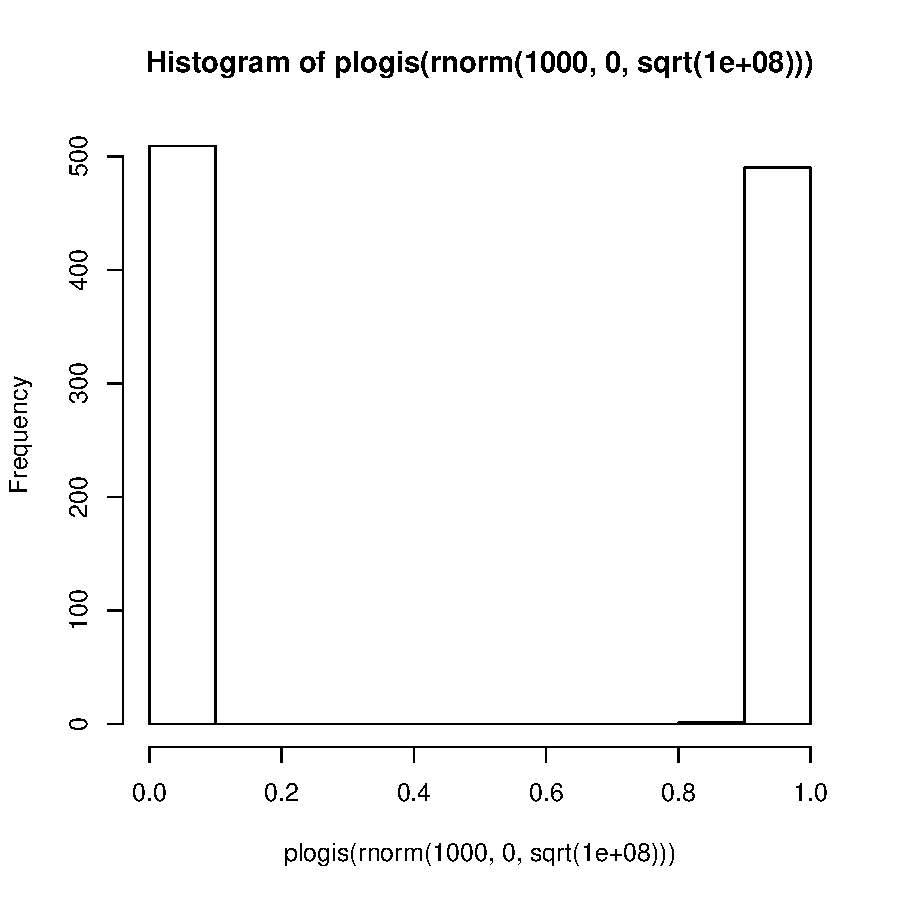
\includegraphics{Lecture2-074}
\end{center}
\caption{Histogram of 1000 random deviates from a normal distribution with a mean of zero and a large variance ($10^8$) after undergoing an inverse logit transformation.}
\label{invlogit-fig}
\end{figure}

This diffuse prior can cause problems if there is complete (or near complete) separation. Generally this happens when the binary data associated with some level of a categorical predictor are all success or all failures. For example, imagine we had 50 binary observations from an experiment with two treatments, for the first treatment the probability of success is 0.5 but in the second it is only one in a thousand:

\begin{Schunk}
\begin{Sinput}
> treatment <- gl(2, 25)
> y <- rbinom(50, 1, c(0.5, 0.001)[treatment])
> data.bin <- data.frame(treatment = treatment, y = y)
> table(data.bin)
\end{Sinput}
\begin{Soutput}
         y
treatment  0  1
        1 13 12
        2 25  0
\end{Soutput}
\end{Schunk}
 
if we analyse using \texttt{glm} we see some odd behaviour:

\begin{Schunk}
\begin{Sinput}
> m2c.1 <- glm(y ~ treatment, data = data.bin, family = "binomial")
> summary(m2c.1)
\end{Sinput}
\begin{Soutput}
Call:
glm(formula = y ~ treatment, family = "binomial", data = data.bin)

Deviance Residuals: 
     Min        1Q    Median        3Q       Max  
-1.14361  -0.85773  -0.00008  -0.00008   1.21159  

Coefficients:
              Estimate Std. Error z value Pr(>|z|)
(Intercept)   -0.08004    0.40032  -0.200    0.842
treatment2   -19.48603 2150.80263  -0.009    0.993

(Dispersion parameter for binomial family taken to be 1)

    Null deviance: 55.108  on 49  degrees of freedom
Residual deviance: 34.617  on 48  degrees of freedom
AIC: 38.617

Number of Fisher Scoring iterations: 18
\end{Soutput}
\end{Schunk}

the effect of treatment does not appear significant despite the large effect size. This is in direct contrast to an exact binomial test: 

\begin{Schunk}
\begin{Sinput}
> m2c.2 <- binom.test(table(data.bin)[2, 2], 25)
> m2c.2
\end{Sinput}
\begin{Soutput}
	Exact binomial test

data:  table(data.bin)[2, 2] and 25 
number of successes = 0, number of trials = 25, p-value = 5.96e-08
alternative hypothesis: true probability of success is not equal to 0.5 
95 percent confidence interval:
 0.0000000 0.1371852 
sample estimates:
probability of success 
                     0 
\end{Soutput}
\end{Schunk}

where the  95\% confidence interval for the probability of success is  0.000 to 0.137.\\

The default \texttt{MCMCglmm} model also behaves oddly (see Figure \ref{separation1-fig}):

\begin{Schunk}
\begin{Sinput}
> prior.m2c.3 = list(R = list(V = 1, fix = 1), G = list(G1 = list(V = 1, 
+     nu = 0.002)))
> m2c.3 <- MCMCglmm(y ~ treatment, data = data.bin, family = "categorical", 
+     prior = prior.m2c.3, verbose = FALSE)
> plot(m2c.3$Sol)
\end{Sinput}
\end{Schunk}



\begin{figure}[!h]
\begin{center}
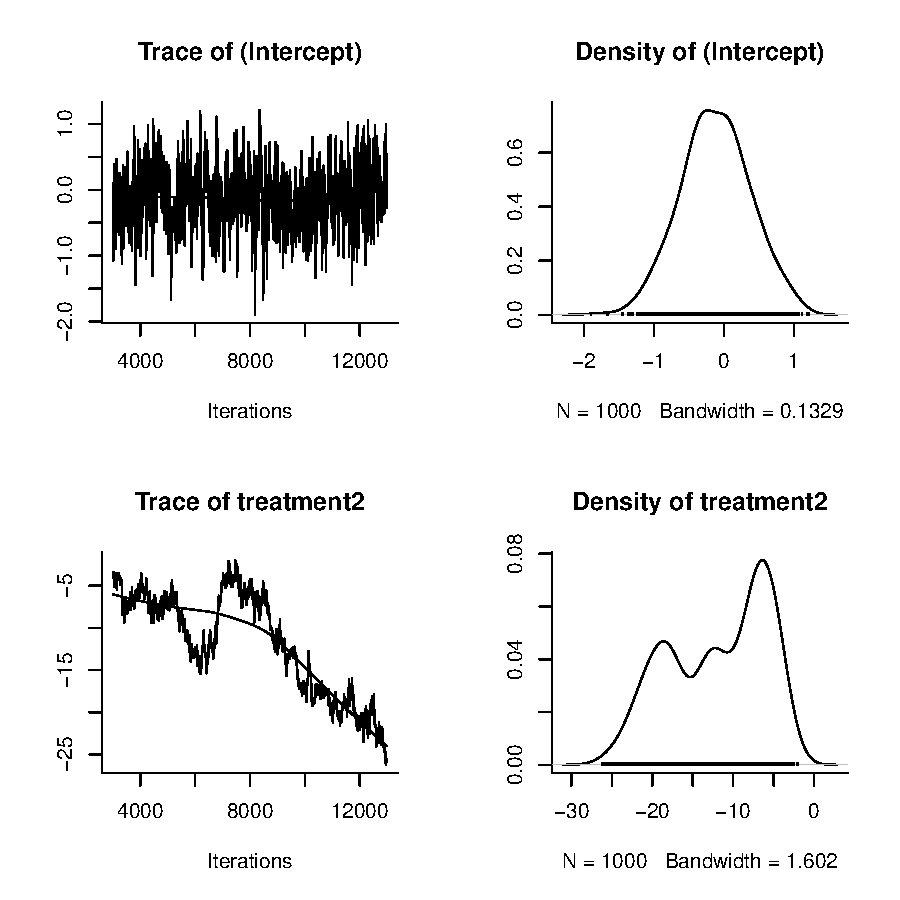
\includegraphics{Lecture2-081}
\end{center}
\caption{MCMC summary plots for the intercept and treatment effect in a binary GLM. In treatment 2 all 25 observations were failures and so the ML estimator on the probability scale is zero and $-\infty$ on the logit scale. With a flat prior on the treatment effect the posterior distribution is improper, and with a diffuse prior (as used here) the posterior is dominated by the high prior densities at extreme values.}
\label{separation1-fig}
\end{figure}

For these types of problems, I usually remove the global intercept (\texttt{-1}) and use the prior $N(0, \sigma^{2}_{\texttt{units}}+\pi^2/3)$ because this is reasonably flat on the probability scale when a logit link is used. For example,

\begin{Schunk}
\begin{Sinput}
> prior.m2c.4 = list(B = list(mu = c(0, 0), V = diag(2) * (1 + 
+     pi^2/3)), R = list(V = 1, fix = 1), G = list(G1 = list(V = 1, 
+     nu = 0.002)))
> m2c.4 <- MCMCglmm(y ~ treatment - 1, data = data.bin, family = "categorical", 
+     prior = prior.m2c.4, verbose = FALSE)
> plot(m2c.4$Sol)
\end{Sinput}
\end{Schunk}


looks a little better (see Figure \ref{separation1-fig}), and the posterior distribution for the probability of success in treatment 2 is consistent with the exact binomial test for which the 95\% CI were (0.000 - 0.137). With such a simple model, the prediction for observation 26 is equal to the  treatment 2 effect and so we can get the the credible interval (on the data scale) for treatment 2 using the predict function:




\begin{figure}[!h]
\begin{center}
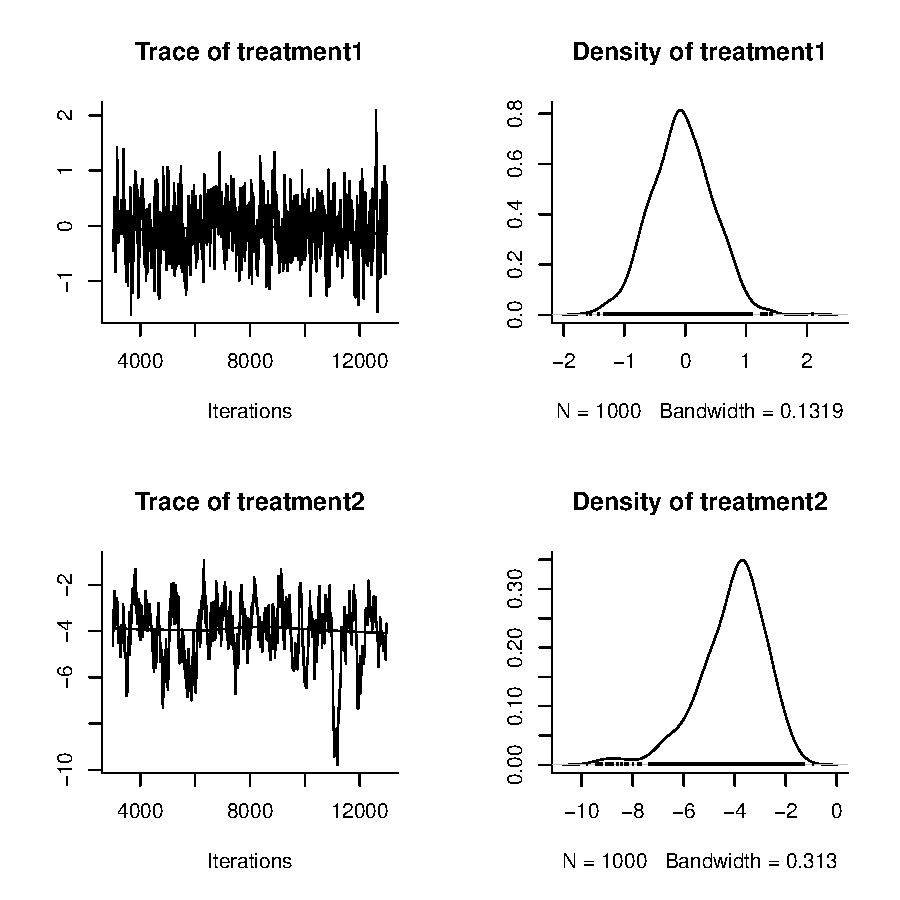
\includegraphics{Lecture2-085}
\end{center}
\caption{MCMC summary plots for the intercept and treatment effect in a binary GLM. In treatment 2 all 25 observations were failures and so the ML estimator on the probability scale is zero and $-\infty$ on the logit scale. A flat prior on the probability scale was used and the posterior distribution is better behaved than if a flat prior on the logit scale had been used (see Figure \ref{separation1-fig}).}
\label{separation2-fig}
\end{figure}

\begin{Schunk}
\begin{Sinput}
> predict(m2c.4, interval = "confidence")[26, ]
\end{Sinput}
\begin{Soutput}
         fit          lwr          upr 
0.0447653495 0.0002971701 0.1296584843 
\end{Soutput}
\end{Schunk}


\section{A note on fixed effect priors and covariances}
\label{PriorContr-sec}

Fixed and random effects are essentially the same thing. The only difference is that the variance component for the fixed effects is usually fixed at some large value, whereas the variance component for the random effects is estimated.  In section \ref{ranef-sec} I demonstrated this by claiming that a model where year effects were fixed (\texttt{m2a.5}) was identical to one where they were treated as random, but with the variance component set to a large value (\texttt{m2a.6}). This was a white lie as I did not want to distract attention from the main point. The reason why they were not identical is as follows:\\

In the fixed effect model (\texttt{m2a.5}) we had the prior:  

\begin{equation}
\begin{array}{rcl}
\left[
\begin{array}{c}
 \beta_{\texttt{(Intercept)}}\\
 \beta_{\texttt{year1962}}\\
\end{array}
\right]
\sim
&
\left[
\begin{array}{cc}
10^8&0\\
0&10^8\\
\end{array}
\right]\\
\end{array}
\end{equation}

Where $\beta_{\texttt{(Intercept)}}$ and $\beta_{\texttt{year1962}}$ are the fixed effects to be estimated.\\

Remembering the identity  $\sigma^{2}_{(a+b)} = \sigma^{2}_{a}+ \sigma^{2}_{b}+2\sigma_{a,b}$, this implies:

\begin{equation}
\begin{array}{rccl}
\left[
\begin{array}{c}
 \beta_{1961}\\
 \beta_{1962}\\
\end{array}
\right]
=
&
\left[
\begin{array}{c}
 \beta_{\texttt{(Intercept)}}\\
 \beta_{\texttt{(Intercept)}}+\beta_{\texttt{year1962}}\\
\end{array}
\right]
\sim
&
\left[
\begin{array}{cc}
10^8&10^8\\
10^8&10^8+10^8\\
\end{array}
\right]
&=
\left[
\begin{array}{cc}
10^8&10^8\\
10^8&20^8\\
\end{array}
\right]\\
\end{array}
\end{equation}

where $\beta_{1961}$ and $\beta_{1962}$ are the actual year effects, rather than the global intercept and the contrast. In hindsight this is a bit odd, for one thing we expect the 1962 effect to be twice as variable as the 1961 effect. With such weak priors it makes little difference, but lets reparameterise the model anyway.\\

 Rather than having a global intercept and a year contrast, we will have separate intercepts for each year:

\begin{Schunk}
\begin{Sinput}
> X3 <- model.matrix(y ~ year - 1, data = Traffic)
> X3[c(1, 2, 184), ]
\end{Sinput}
\begin{Soutput}
    year1961 year1962
1          1        0
2          1        0
184        0        1
\end{Soutput}
\end{Schunk}

and a prior that has a covariance between the two year effects:

\begin{Schunk}
\begin{Sinput}
> PBV.yfixed <- diag(2) * 1e+08
> PBV.yfixed[1, 2] <- PBV.yfixed[2, 1] <- 1e+08/2
> PBV.yfixed
\end{Sinput}
\begin{Soutput}
      [,1]  [,2]
[1,] 1e+08 5e+07
[2,] 5e+07 1e+08
\end{Soutput}
\begin{Sinput}
> prior.m2a.5.1 <- list(B = list(mu = rep(0, 2), V = PBV.yfixed), 
+     R = list(V = 1, nu = 0.002))
\end{Sinput}
\end{Schunk}

This new model:

\begin{Schunk}
\begin{Sinput}
> m2a.5.1 <- MCMCglmm(y ~ year - 1, family = "poisson", data = Traffic, 
+     prior = prior.m2a.5.1, verbose = FALSE)
\end{Sinput}
\end{Schunk}

has the same form as a mixed effect model with a prior variance of $\frac{10^{8}}{2}$ for the intercept, and the variance component associated with the random year effects also fixed at $\frac{10^{8}}{2}$:

\begin{Schunk}
\begin{Sinput}
> prior.m2a.6.1 <- list(B = list(mu = 0, V = 1e+08/2), R = list(V = 1, 
+     nu = 0.002), G = list(G1 = list(V = 1e+08/2, fix = 1)))
\end{Sinput}
\end{Schunk}


This arises because the two random effects have the joint prior distribution:

\begin{equation}
\begin{array}{rl}
\left[
\begin{array}{c}
 \beta_{\texttt{year.1961}}\\
 \beta_{\texttt{year.1962}}\\
\end{array}
\right]
\sim
&
\left[
\begin{array}{cc}
\frac{10^{8}}{2}&0\\
0&\frac{10^{8}}{2}\\
\end{array}
\right]\\
\end{array}
\end{equation}

which when combined with the prior for the intercept, $N(0, \frac{10^{8}}{2})$, gives:

\begin{equation}
\begin{array}{rccl}
\left[
\begin{array}{c}
 \beta_{1961}\\
 \beta_{1962}\\
\end{array}
\right]
=
&
\left[
\begin{array}{c}
 \beta_{\texttt{(Intercept)}}+\beta_{\texttt{year.1961}}\\
 \beta_{\texttt{(Intercept)}}+\beta_{\texttt{year.1962}}\\
\end{array}
\right]
\sim
&
\left[
\begin{array}{cc}
\frac{10^{8}}{2}+\frac{10^{8}}{2}&\frac{10^{8}}{2}\\
\frac{10^{8}}{2}&\frac{10^{8}}{2}+\frac{10^{8}}{2}\\
\end{array}
\right]
&=
\left[
\begin{array}{cc}
10^8&\frac{10^{8}}{2}\\
\frac{10^{8}}{2}&10^8\\
\end{array}
\right]
\\
\end{array}
\end{equation}

which is equivalent to the \texttt{PBV.yfixed} parameteristaion of for the two years.\\

The model:

\begin{Schunk}
\begin{Sinput}
> m2a.6.1 <- MCMCglmm(y ~ 1, random = ~year, family = "poisson", 
+     data = Traffic, prior = prior.m2a.6.1, verbose = FALSE, pr = TRUE)
\end{Sinput}
\end{Schunk}

is therefore sampling from the same posterior distribution as model \texttt{m2a.5.1}.
\ifalone
\end{document}
\else
\fi



